\documentclass{sig-alternate}

\usepackage[utf8]{inputenc}
\usepackage{texgraphicx}
\graphicspath{{fig/}}
\usepackage{multirow}
\usepackage{multicol}
\usepackage{xspace}
\usepackage{amsfonts,amsmath,amssymb,amstext,latexsym,stmaryrd}
\usepackage{url}
\usepackage{boxedminipage}
\usepackage{subfigure}

\usepackage{manfnt}
\newcommand{\danger}{\marginpar[\hfill\dbend]{\dbend\hfill}}
\newcommand{\FIXME}[1]{%
  \begin{center}
    \dbend%
    \begin{boxedminipage}{.8\linewidth}
      #1
    \end{boxedminipage}
    \dbend%
  \end{center}
}%

\def\etc{, etc.\xspace}
\def\ie{i.e.,\xspace}
\def\eg{e.g.,\xspace}
\def\cf{cf.\xspace}
\def\etal{\emph{et al.}\xspace}


\makeatletter
\newcommand{\eqnlabel}[1]{\xdef\@currentlabel{\theequation}\ltx@label{#1}}
\newcommand{\cnstslabel}[2][\thesubcounstraints]{
  \refstepcounter{subcounstraints}%
  \xdef\@currentlabel{#1}%
  \tagform@{#1}%
  \ltx@label{#2}\quad &}

\newcommand{\cnstslabelBIS}[2][\thesubcounstraints]{
  \refstepcounter{subcounstraints}%
  \xdef\@currentlabel{#1}%
  \tagform@{#1}%
  \ltx@label{#2}\quad }

%\newcommand{\cnstslabel}[1]{\ltx@label{#1}}
\newcounter{subcounstraints}[equation]

\newenvironment{LinearProgram}[2][Maximiser]{%
  \begin{equation}%
    \let\label=\eqnlabel
    \begin{array}{l}%
      \textsc{#1 } #2, \\%
      \textsc{under constraints}\\%
      \begin{cases}%
}{%
      \end{cases}
    \end{array}
  \end{equation}%
}

\newcommand{\EquationsNumbered}[1]{%
  \setcounter{subcounstraints}{0}
  \renewcommand{\thesubcounstraints}{\theequation\alph{subcounstraints}}
  \def\set@counstraintscounter{
    \refstepcounter{subcounstraints}%
    \xdef\@currentlabel{\thesubcounstraints}%
    \tagform@{\thesubcounstraints}%
  }
  \def\mark{\set@counstraintscounter\quad&}
  \def\n{\\\mark}
  \begin{aligned}%
    #1
  \end{aligned}%
}
\makeatother

\def\alvinbreak{\discretionary{}{}{}}
\def\sec{\ensuremath{\text{sec}}\xspace}%
\def\ms{\ensuremath{\text{ms}}\xspace}%
\def\MBps{\ensuremath{\text{MB}/\text{s}}\xspace}%
\def\MB{\ensuremath{\text{MB}}\xspace}%
\def\KBps{\ensuremath{\text{KB}/\text{s}}\xspace}%
\def\KB{\ensuremath{\text{KB}}\xspace}%

\let\leq=\leqslant
\let\geq=\geqslant


\begin{document}

\conferenceinfo{SIMUTools}{'09, Rome, Italy}
\CopyrightYear{2009}
\crdata{978-963-9799-45-5}

\title{Accuracy Study and Improvement of Network Simulation in the
  SimGrid Framework}
% \titlenote{An extended version of this paper is available as
%   INRIA research report~\cite{RR-FIXME}}

\numberofauthors{2}
\author{
\alignauthor
\mbox{Pedro Velho}\\
       \affaddr{University of Grenoble -- INRIA MESCAL Project}\\
       \affaddr{LIG Laboratory - ENSIMAG - 51 Avenue
         Jean Kuntzmann - 38330 MontBonnot Saint-Martin - France}\\
       \email{pedro.velho@imag.fr}
% 2nd. author
\alignauthor
Arnaud Legrand\\
       \affaddr{CNRS -- University of Grenoble -- INRIA MESCAL Project}\\
       \affaddr{LIG Laboratory - ENSIMAG - 51 Avenue
         Jean Kuntzmann - 38330 MontBonnot Saint-Martin - France}\\
       \email{arnaud.legrand@imag.fr}
}

\maketitle

\newcommand{\simgrid}{SimGrid\xspace}%
\newcommand{\gtnets}{GTNetS\xspace}%
\begin{abstract}
  Distributed computing is a very broad and active research area
  comprising fields such as cluster computing, computational grids,
  desktop grids and peer-to-peer (P2P) systems. Studies in this area
  generally resort to simulations, which enable reproducible results
  and make it possible to explore wide ranges of platform and
  application scenarios.  In this context, network simulation is
  certainly the most critical part. 
  Many packet-level network simulators are
  available and enable high-accuracy simulation but they lead to
  prohibitively long simulation times. Therefore, many simulation
  frameworks have been developed that simulate networks at higher
  levels, thus enabling fast simulation but losing accuracy.  One such
  framework, \simgrid, uses a flow-level approach that approximates
  the behavior of TCP networks, including TCP's bandwidth sharing
  properties. A preliminary study of the accuracy loss by comparing it
  to popular packet-level simulators has been proposed
  in~\cite{nstools07} and in which regimes in which \simgrid's accuracy
  is comparable to that of these packet-level simulators are
  identified. In this article we come back on this study, reproduce
  these experiments and provide a deeper analysis that enables us to
  greatly improve \simgrid's range of validity.
\end{abstract}

% A category with the (minimum) three required fields
\category{I.6.4}{Model Validation and Analysis}{Network Simulation}
%A category including the fourth, optional field follows...
\category{I.6.7}{Simulation Support System}{\simgrid,\gtnets}

\terms{Network Simulation}

%\keywords{} % NOT required for Proceedings

\section{Introduction}

In the last few decades, considerable breakthroughs in eScience,
peer-to-peer and collaborative computing have been achieved.  These
emerging technologies are however based on the connection of thousands
of resources through a wide area network. Hence such systems have a
dramatically increasing conception complexity and research in this area
generally boils down to the development of better systems and algorithms.

Evaluating the merit of alternative designs or solutions is hard for
many reasons. First, real experiments on such large-scale distributed
platforms are considerably time consuming. Second, network devices and
software have many possible standards an implementations, leading to
different behaviors and interactions that are very difficult to
control. Thus, such systems are so complex and unstable that
experiments are not repeatable. Last, it is generally very hard to
obtain such platforms at hand to execute experiments. That is why most
research in this area resort to simulation-based studies.

Simulation is, in its essence, the act of imitating the behavior of some
process. More specifically, in the computer science research field,
simulation amounts to implement a model, that is to say, 
a hypothetical description of the system (\eg an equation system, a
state-automata, a Petri net, \dots). %  Generally
% speaking, a model can be: an equation system, a program, a Petry net,
% among others. Also, different models can be combined in order to
% provide more complex one. 
In many aspects the simulation approach offers attractive
properties. First, simulations are repeatable, which is generally not
the case of experiments on real distributed systems because of their
unstability and of their complexity. Second, simulations are
configurable, meaning that they provide a way of testing hypothetical
parameters or platforms hence enabling to try many alternative designs
and to extrapolate on future scenarios. Last but not least, simulations
provide fast results, thus avoiding common misconception
alternatives.

Although simulation speed is desired, it is often achieved at the cost
of accuracy loss. For instance, analytical models
generally provide fast approximations but they rarely have more
accurate results than event-driven simulations. Investigating this
accuracy/speed tradeoff is frequently neglected, particularly in
large-scale distributed platforms simulation. Yet, accuracy is mandatory to avoid severe bias in simulation analysis. Generally,
models are valid only for a limited range of parameters and surprisingly,
despite the importance of this validity range, this information is not
easily found for most popular distributed computing simulators.

Focusing in distributed platforms simulation, the
network part is indubitably the most critical and controversial part.
Every user needs to drive fast simulations involving thousands of
transfer of arbitrary size and expects accurate results.  In the
network domain, the most accurate tools to study protocols are known
as packet-level simulators. Such simulators implement an event
driven model passing through all protocol layers and are thus
generally recognized as accurate. They are however extremely slow, which
makes them useless for everyday simulation of large-scale distributed
systems. Therefore, higher-level simulations are thus generally
used. GridSim~\cite{REF_35} uses a variable size packet-level
simulation (which is quite slow and whose realism remains to be
proved) while OptorSim~\cite{REF_2} and \simgrid~\cite{simgrid} use a
flow-level simulation. However OptorSim sharing mechanism is known to
be unrealistic in very simple settings. Still, such tools are commonly
used and very few users question their relevance, which is why many
people criticize simulation as a whole without distinguishing between
the different approaches.

Note that in experimental science the act of reproducing past
results is mandatory to obtain universal and enduring knowledge.
Such a feature is commonly found in all classic
sciences such as physics, medicine or chemistry. However, in computer science
the fact of reproducing experiments is rarely seen as a fundamental
step and most published work focus on novelty and performance.
Reproducing the results of others is even sometimes
interpreted as waste of time. Still, we claim that such an
unattractive work is important and enables either to confirm or to
refute previous results.

Therefore, in this article, we focus on the accuracy analysis of network
simulation within the \simgrid framework by reproducing past experiments.
Fujiwara\etal~\cite{nstools07} have proposed a preliminary
study of the accuracy of the \simgrid model comparing obtained results
with packet-level simulations and have highlighted non-neglectable
flaws. In this article, we come back on their study and improve on
their results by making a finer analysis that enables us to propose a
more accurate model at very low cost. More precisely, our contributions
are the following:

\begin{itemize}
\item We reproduce and confirm the results of~\cite{nstools07} but
  using a more precise and well-suited error model. We also use a more
  unified and justified protocol running more experiments than
  what was previously done.
\item We propose a finer analysis than the one proposed
  in~\cite{nstools07} and we study more precisely the validity range
  of the \simgrid model.
\item This finer analysis reveals that some parameters of the \simgrid
  model were incorrectly instantiated and that a few simple
  modifications enable to greatly improve its accuracy, which we
  evaluate through the same protocol.
\end{itemize}

This article is organized as follows:

\begin{itemize}
\item In Section~\ref{sec.related}, we briefly present packet-level
  simulation and flow-based simulation. We also briefly present the
  main characteristics of the \simgrid model. Then, we present the
  three case studies performed in~\cite{nstools07} and the evaluation
  methodology they used. Last, we present their conclusion on the
  validity of the \simgrid model.
\item In Section~\ref{sec.onelink}, we present our analysis of the
  first case study: predicting the completion time of a single
  communication going through a single link. We propose and justify a
  new error model and explain how to improve this error and thus
  increase the validity range to smaller messages and more diverse
  bandwidth and latencies parameters.
\item In Section~\ref{sec.dogbone}, we present our analysis of the
  second case study: predicting the bandwidth sharing of two
  communications competing on a dumbbell topology. We propose a more
  precise evaluation protocol and show that the error model seamlessly
  extends to this new situation. A careful study of the relation
  between the accuracy and the platform parameters enables to identify
  a flaw in the model instantiation. We propose a slightly different
  model and explain how to instantiate it correctly. Last, we study its
  accuracy and its validity range.
\item In Section~\ref{sec.random}, we present our analysis of the
  third case study: predicting the bandwidth sharing of many flows
  competing on a random topology. Once again, we reproduce the
  experiments of~\cite{nstools07} but with a more precise evaluation
  protocol and error model. We show that the new model always improves
  on the previous model and we present the magnitude of accuracy gain.
\item Last, in Section~\ref{sec.conclusion} we draw some conclusion
  and present some leads to further improve the \simgrid model.
\end{itemize}

\section{Related Work}
\label{sec.related}

Section~\ref{sec:rel.packet} and~\ref{sec:rel.flow} present general
content on packet-level and flow-level simulation already presented
in~\cite{nstools07} by Fujiwara \etal but included here for
completeness\footnote{Fujiwara and Casanova kindly allowed us to
  reproduce their material that could, in our opinion, hardly be
  improved.}. The main difference is that
Section~\ref{sec:rel.flow} slightly more details models
with mathematical notations to explain more precisely model
modifications proposed in Section~\ref{sec.onelink}
and~\ref{sec.dogbone}. Section~\ref{sec:rel.kayo} briefly summarize
the experiments and the conclusions presented in~\cite{nstools07}.

\subsection{Packet-Level Simulation}
\label{sec:rel.packet}
Packet-level simulators use discrete-event simulation by which a flow
over a network path can be represented as a sequence of events, such
as packet arrivals and departures at end-points and
routers. End-points and routers both implement full-fledge network
protocols. Simulation time typically increases in proportion to the
number of events~\cite{REF_15}.  Popular such simulators include
ns-2~\cite{REF_22}, \gtnets~\cite{REF_29}, and
SSFNet~\cite{REF_6}. As mentioned in the introduction, the main
problem with these simulators is that simulation time can be orders of
magnitude larger than simulated time for simulations that involve
realistic topologies with many flows. For instance, using \gtnets, which
is known for good scalability, simulating 200 flows each transferring
100\MB between two random end-points in a random 200-node topology for
125 \sec of simulated time takes approximately 1500 \sec on a 3.2GHz
Xeon processor~\cite{nstools07}. While this is acceptable for
researchers studying network protocols, it is prohibitive for many
researchers studying distributed systems and algorithms on large-scale
platforms for application that are long-running and/or that involve
large amounts of communication. This problem is often compounded by
the need to rely on results from over thousands of simulation
experiments to compute valid statistics regarding the relative
effectiveness of competing algorithms, which uses over one million
simulation experiments, with each experiments requiring over 1,000
\sec of simulated time).

Several researchers have attempted to increase the speed of
packet-level simulations. For instance, in~\cite{REF_16} the authors
developed the MaSSF framework, which combines the DaSSF packet-level
simulator~\cite{REF_5} with message passing~\cite{REF_33} to
accelerate and increase the scalability of network simulation by
running in parallel on large clusters of workstations. MaSSF is the
main component of the MicroGrid~\cite{REF_34} tool for simulating Grid
platforms and applications. Others have proposed emulation techniques
by which traffic flows on physical devices, introducing delay, bandwidth
and packet loss characteristics of the network to be simulated. A
well-known example of such work is ModelNet~\cite{REF_38}.


While the last mentioned works do increase the speed and scalability of
packet-level simulation without compromising simulation accuracy, many
users performing grid simulations need simulations orders of magnitude
faster. Facing such requirements, simulators that relax the
definition of a packet were developed. For instance, the Bricks
simulator~\cite{REF_36} uses ideal queuing networks to simulate real
networks. While the user can specify a packet size in this simulator,
Bricks packets do not correspond to real network packets and Bricks
does not implement real network protocols. Large packets lead to fast
simulation but obviously low accuracy (in the extreme, multi-path
network communications use a store-and-forward approach with no
pipelining across network links). Although lower packet size leads to
behavior presumably qualitatively closer to that of real networks,
nothing in this simulator ensure that the behavior is quantitatively
close to that of, for instance, TCP. Another simulator,
GridSim~\cite{REF_35} implements a protocol that includes some
elements of UDP and allows for variable packet size. Like Bricks,
GridSim requires small packet size to hope to gain accuracy close to
that of true packet-level simulators on realistic network topologies,
but then suffers from high simulation costs. Many other ``grid''
simulators exist, such as OptorSim~\cite{REF_2},
GangSim~\cite{REF_7}, Neko~\cite{REF_25}, or
HyperSim~\cite{REF_27} (readers interested in depth details are invited to consult~\cite{REF_28}). All
implement some network model, but to the best of our knowledge (i.e.,
based on publications and/or on inspection of source codes), these
simulators either use packet-level simulation or do not attempt to
implement a model that realistically tracks the behavior of TCP
networks.

\subsection{Flow-based Simulation}
\label{sec:rel.flow}
\def\L{\ensuremath{\mathcal{L}}\xspace}%
\def\F{\ensuremath{\mathcal{F}}\xspace}%
To increase the speed of network simulation one approach is to use
theoretical models to compute the throughput of each flow in a network
topology at a given time. 
Models have been proposed~\cite{REF_26,
  REF_19, REF_24} that model the throughput of a TCP flow as a
function of packet loss and round trip delay, as well as some
parameters of the network and of the TCP protocol. Unfortunately, some
of these parameters are difficult to measure and/or instantiate for
the purpose of grid simulations. Furthermore, it is not clear how the
model can be applied to arbitrary network topologies with many
simulated flows competing for network resources. Instead, one desires
reasonable models that capture the bandwidth sharing behavior induced
by TCP among flows on arbitrary topologies and that are defined by a
few simple parameters, namely link physical bandwidths and TCP
congestion window size.  This definition of macroscopic models of
bandwidth sharing is challenging~\cite{REF_18}.
These models generally fit in the following
framework. Every link $\L_k$ has a maximum bandwidth $B_k$ and every
flow $\F_i$ has a throughput $\rho_i$ and we need to ensure that the
capacity $B_k$ of each link is never exceeded. Therefore, the system
is generally defined with the following constraints.
\begin{equation*}
  \forall \L_k: \sum_{i | \F_i \text{ uses } \L_k} \rho_i \leq B_k
\end{equation*}
A key question is then: which type of ``fairness'' does TCP implement when
flows share bandwidth on bottleneck links? 
The most widely known model is
the simple Max-Min fairness model~\cite{BG92}, which computes a
bandwidth allocation in which increasing the allocation of
a flow would require decreasing the allocation of another.
However, it is well-known that TCP does not implement
Max-Min fairness, as shown for instance by Chiu~\cite{REF_4}. 

Indeed, the analytical models for TCP throughput in~\cite{REF_8,
  REF_26} approximate the throughput, $\rho(p)$, to $\rho(p)=c/(RTT.\sqrt{p})$
where $p$ is the fraction of packets lost, $RTT$ is the round-
trip time, and $c$ is some constant, provided that $p$
is not ``too high''. Assuming that all flows experience the
same loss rate, $p$, this formula suggests that bandwidth is
in fact shared in inverse proportion to the RTT. This thus
suggests a Max-Min scheme that is modified to account for
low RTTs. 
Additionaly, the TCP congestion mechanism relies on a window whose
size is generally bounded (we denote by $W$ this maximum window size),
which impacts greatly the effective bandwidth of the flows (the
effective throughput is thus bounded by $W/RTT$ as there are always at
most $W$ pending packets).

Last, it has been proved that TCP sharing mechanism at the equilibrium
is indeed equivalent to maximizing
\begin{equation}
\sum_i
\frac{\sqrt{3/2}}{D_i}\tan^{-1}(\sqrt{3/2}D_i\rho_i),
\label{eq.low}
\end{equation}
where $D_i$ is
the equilibrium round-trip-time~\cite{Low03}. Such an equilibrium is
generally different from the max-min sharing and should thus be more
accurate. Solving such equations is however harder than the max-min
sharing algorithm.

Based on the previous considerations, the designer of the \simgrid
simulation tool~\cite{simgrid, simgrid_website}, have opted for a RTT-aware
Max-Min flow-level model. In this model, the bandwidths allocated to
flows competing over a bottleneck link is inversely proportional to
the flows' RTTs (A link is considered a bottleneck if the sum of the
bandwidths allocated to the flows over this link is equal to the total
bandwidth of the link.) and the bandwidth of each flow is bounded by a
value inversely proportional the inverse of its RTT.

\begin{LinearProgram}[Maximize]{\min_i RTT_i.\rho_i}
  \EquationsNumbered{
    \cnstslabel{eq.link_bound} \forall \L_k, \sum_{i | \F_i \text{
        uses } \L_k}
    \rho_i \leq B_k\\
    \cnstslabel{eq.flow_bound} \forall \F_i, \rho_i \leq \frac{W}{RTT_i}
  }
\end{LinearProgram}

We refer the reader to~\cite{RR-Loris} for full details on
the model and for initial validation results via which this
particular model was selected among several alternatives. The model is
instantiated solely based on network link physical characteristics
(latencies and bandwidths) and on the size of the TCP congestion
window size. As a result, \simgrid is, to the best of our knowledge,
the first simulation framework designed for the study of distributed
systems and algorithms for large-scale platforms that uses a flow-level
network simulation approach that attempts to capture the true
behavior of TCP networks and that decreases simulation costs by orders
of magnitude when compared to packet-level simulation.

\subsection{Flow-level Simulation Accuracy}
\label{sec:rel.kayo}
Although \simgrid has garnered a sizeable user base, its flow-level
network simulation scheme has several limitations.  It does not
capture the slow-start feature of TCP. Instead, it assumes that flows
are backlogged and in steady state.  Also, it assumes that the RTT of
each flow is constant and is equal to twice the sum of the link
latencies on the flow's network path. And of course, the model cannot
account for any detail pertaining to the behavior of individual
packets.  Therefore, one may wonder how accurate the network
simulation in \simgrid is. For instance, the simulation of short TCP
flows should incur large inaccuracies since slow-start is not accounted
for. 

Fujiwara\etal~\cite{nstools07} had quantified such inaccuracy
and identified regimes in which simulation results deviate signicantly
from those of packet-level simulation performed with GTNets. One of
the aim of the present article is to reproduce and provide a finer
analysis of their results. To this end, we briefly recall the
experiments that were conducted in~\cite{nstools07}:
\def\BOneLink{\ensuremath{\mathbf{B}}\xspace}%
\def\LOneLink{\ensuremath{\mathbf{L}}\xspace}%
\def\BDogbone{\ensuremath{\mathbf{B}}\xspace}%
\def\LDogbone{\ensuremath{\mathbf{L}}\xspace}%
\begin{description}
\item[One Link] The first set of experiments is for a single TCP flow
  going through a single link with physical latency $\LOneLink\in \{0,
  1, 10, 20, 40, 60, 80, 100\}$ (in \ms) and physical bandwidth
  $\BOneLink\in\{0.1, 0.2, 0.4, 0.6, 0.8, 1, 10, 100, 10\,000\}$ (in
  \MBps). The TCP senders send $S\in\{0.001, 0.01, 0.1, \alvinbreak 1,
  10, 100, 1000\}$ \MB of data to the receivers and the communication
  time is measured with GTNets and with the \simgrid model.

  The conclusions of these experiments are that \simgrid achieves
  accuracy comparable to the packet-level simulators (\ie the
  relative throughput differs at most by 1\%) for message size
  $S>10\MB$. For smaller data sizes the throughput by the \simgrid
  simulation is much higher (\eg a factor 5) than those by the
  packet-level simulation.  Indeed, the network model in \simgrid
  assumes that TCP flows are in steady-state so that the 
  TCP slow-start mechanism is negligible. This assumption is realistic
  for large data sizes, but breaks down for small data sizes. 
\item[Dumbbell Topology] The second set of experiments is for two TCP
  flows $A$ and $B$ on a dumbbell topology defined by two parameters
  $\BDogbone\in\{0.1, 100\}$ (in \MBps) and $\LDogbone\in \{0, 1, 5,
  10,20, 50,100\}$ (in ms) as depicted in Figure~\ref{fig:dogbone}.
  \begin{figure}
    \centering
    \includegraphics[width=\linewidth]{dogbone.fig}
    \caption{Dumbbell Topology}
    \label{fig:dogbone}
  \end{figure}
  The experiments were conducted with a message size $S$ equal to
  100\MB to avoid the inaccuracy issues raised in the first set of
  experiments. The effective throughput (\ie the message size divided
  by total communication time) for each flow was then measured with
  both \simgrid and \gtnets.

  The conclusions of these experiments are that \simgrid achieves
  accuracy comparable to the packet-level simulators (\ie the
  relative throughput differs at most by 1\%) when the capacity of the
  middle link is large (\ie for $\BDogbone = 100\MBps$). This
  corresponds to the fact that both flows are bounded by the
  inverse of their round-trip time (\ie by
  constraint~\eqref{eq.flow_bound}). However when the throughput get
  limited by the physical bandwidth (\ie for $\BDogbone = .1 \MBps$)
  there is an important discrepency between \simgrid and \gtnets, even
  though trends are respected (the flow with the larger RTT achieves a
  lower throughput than the flow with the lower RTT).

\item[Random Topology] The third set of experiments is for random
  flows on random topologies. Four sets of 10 random topologies were
  generated with the Waxman model~\cite{Waxman88} and the BRITE
  generator~\cite{brite}. The sets comprised either small (50 nodes)
  or large (200 nodes) and either homogeneous ($B\in [100,128]$ \MBps)
  or heterogeneous ($B\in [10,128]$ \MBps) platforms. 200 flows were
  generated between random pairs of end-points in the topology, which
  all start simultaneously and communicate 100\MB of data. Once again,
  the effective throughput (\ie the message size divided by total
  communication time) for each flow was then measured with both
  \simgrid and \gtnets.

  The conclusion of these experiments is that the accuracy of \simgrid
  is correlated to the contention in the network. For experiments with
  low contention (\ie generally those involving many nodes
  and a rather high bandwidth), 80\% of flows have a relative error
  smaller than 1\% while the throughput of the other flows are
  over-estimated or under-estimated. For experiments with high
  contention (\ie generally those with only a few nodes and rather
  low bandwidth) only 20\% of flows have a relative error
  smaller than 1\%.
\end{description}

\begin{table*}
  \begin{center}
    \begin{minipage}[t]{.45\linewidth}
      \caption{Logarithmic error analysis of linear model with
        \gtnets.}
      \label{tab.1link_sg}
      \begin{center}
        \begin{tabular}{c|c|c|c}
          \hline
          Size $\geq$ & \multicolumn{3}{c}{Logarithmic Error}   \\ \cline{2-4}
          & Max & Mean &  Sd   \\ \hline
          1 \KB & 1.8539 & 0.6235 & 0.6296 \\ 
          10 \KB & 1.6771 & 0.4087 & 0.5103 \\
          100 \KB & 0.6650 & 0.1270 & 0.1450 \\
          1 \MB & 0.1474 & 0.0464 & 0.0237 \\
          10 \MB & 0.0662 & 0.0372 & 0.0265 \\
          100 \MB & 0.0609 & 0.0365 & 0.0270 \\ \hline
        \end{tabular}
      \end{center}
    \end{minipage}
    \hfil
    \begin{minipage}[t]{.45\linewidth}
      \caption{Improved linear model versus \gtnets.}
      \label{tab.1link_new}
      \begin{center}
        \scalebox{0.90}{\begin{tabular}{c|c|c|c|c|c} \hline Size
            $\geq$ & $\alpha$ & $\beta$ &
            \multicolumn{3}{c}{Logarithmic Error} \\ \cline{4-6} & & &
            Max & Mean & Sd \\ \hline
            1   \KB & 0.6000  & 6.2400   & 0.4359 & 0.1710 & 0.1373 \\
            10  \KB & 0.7666  & 8.5008   & 0.1803 & 0.0478 & 0.0559 \\
            100 \KB & 0.9200  & 10.4000  & 0.0634 & 0.0108 & 0.0149 \\
            1   \MB & 0.9202  & 14.8193  & 0.0481 & 0.0117 & 0.0105 \\
            10  \MB & 0.9056  & 22.4166  & 0.0077 & 0.0022 & 0.0027 \\
            100 \MB & 0.8976  & 22.4166  & 0.0010 & 0.0005 & 0.0004 \\

            \hline
          \end{tabular}}
      \end{center}
    \end{minipage}
  \end{center}
\end{table*}

The main conclusions of this study are that the \simgrid model is
orders of magnitude faster than packet-level and that
its accuracy would likely becomes unacceptable for many users when
data sizes are ``small'' (due to the TCP slow-start mechanism) or when
networks are ``highly contended'' (i.e., low physical bandwidths
and/or many flows). The ``small'' message issue is important as soon
as message size is smaller than 10\MB but seemed a necessary evil
coming from the stationary flow assumption. The contention issue
could be explained by the fact that the Max-Min sharing mechanism
(even if simple to implement) does not realistically  model the complex TCP
sharing mechanism, which pointed toward alternative solutions like
optimizing~\eqref{eq.low} with techniques like Lagrangien optimization.

By carefully reproducing these experiments and analyzing more
precisely their result, we show that these two issues can be greatly
addressed at low cost.

\newpage
\section{One Link}
\label{sec.onelink}
\newcommand{\tGT}[1][]{\ensuremath{T_{#1}^{(GT)}}\xspace}
\newcommand{\tSG}[1][]{\ensuremath{T_{#1}^{(SG)}}\xspace}
\newcommand{\tSGN}[1][]{\ensuremath{T_{#1}^{(new)}}\xspace}
\newcommand{\thGT}[1][]{\ensuremath{Th_{#1}^{(GT)}}\xspace}
\newcommand{\thSG}[1][]{\ensuremath{Th_{#1}^{(SG)}}\xspace}
\newcommand{\thSGN}[1][]{\ensuremath{Th_{#1}^{(new)}}\xspace}

Besides the evaluation of \simgrid accuracy, the other major
contribution of Fujiwara\etal~\cite{nstools07} is the integration of
\gtnets within \simgrid. The same \simgrid code can use either the
standard Max-Min model or run in a packet-level simulation mode that
use \gtnets, which greatly eases our study.

We have reproduced the ``One Link'' experiments with a slightly larger
set of parameters. More precisely, we have geometrically sampled the
interval $[0.001,600]$ (in \MB) with 165 points for the message size
$S$. We have geometrically sampled the interval $[0.01,500]$ (in \ms)
with 16 points for the latency \LOneLink. Last, we have geometrically
sampled the interval $[0.01,500]$ (in \MBps) with 43 points for the
bandwidth \BOneLink. Exploring the simulation results shows that,
unsurprisingly, for any latency and bandwidth the \gtnets
communication time \tGT[\LOneLink,\BOneLink] is well approximated by a
linear function of message size.

In such a simple setting the \simgrid communication time
\tSG[\LOneLink,\BOneLink] simply writes as follows:
\begin{equation}
  \label{eq:t_sg}
  \tSG[\LOneLink,\BOneLink](S) = \LOneLink +
  \frac{S}{\min\left(\BOneLink, \frac{W}{2\LOneLink}\right)},
\end{equation}
where $W=20000$ is the maximum window size (the same value as the
default \gtnets value). A careful study of the results reveals that
the previous formula is indeed a good model of
\tGT[\LOneLink,\BOneLink] (and particularly the term
$\frac{W}{2\LOneLink}$) but that it could be slightly improved by
simply adding two correction factors $\alpha$ and $\beta$:
\begin{equation}
  \label{eq:t_sg_new}
  \tSGN[\LOneLink,\BOneLink](S) = \alpha.\LOneLink +
  \frac{S}{\min\left(\beta.\BOneLink, \frac{W}{2\LOneLink}\right)},
\end{equation}

Before explaining how to compute these values $\alpha$ and $\beta$, we
need to properly define an error measure. In~\cite{nstools07}, the
error is computed as a relative difference of throughputs, \ie by:
\begin{equation}
  \label{eq:rel_err}
  Err = \frac{\thSG-\thGT}{\thGT}\text{, where } 
  \thGT=\frac{S}{\tGT(S)}
\end{equation}
The error of a given experiment (\ie a latency, a bandwidth and a
message size) is thus null if and only if both communication times are equal. We
think that this error definition has a few biases. First, the relative
difference of throughputs is different of the relative difference of
communication times and there is a priori no reason to favor
throughputs to communication times. Second, this error measure is not
symetric: the error lies in the interval $(-1,+\infty)$. When
$\tSG=2\tGT$ we get an error of 1 (\ie 100\%) whereas when
$\tSG=\tGT/2$, we get an error of -1/2 (\ie -50\%). Therefore, as we
are more interested by multiplicative errors instead of additive
errors, we propose to compute the error with a logarithmic difference:
\begin{equation}
  \label{eq:rel_err_new}
  \begin{split}
    LogErr & = |\log(\thSG)-\log(\thGT)| \\
    & = |\log(\tGT)-\log(\tSG)|
  \end{split}
\end{equation}
This error measure solves both previous issues: it is invariant when
applied to throughputs or to communication times and is completely
symmetrical. Additionally, one can then apply additive aggregation
operators like the maximum, the mean or the variance. However to
interpret them as a percentage, we need to go back from the
``log''-space. For small values, this can simply be done by
multiplying this value by $100$ but for large values, this would
greatly underestimate the error. For instance, a logarithmic error of
$0.01$ corresponds to a $\exp(0.01)-1=1\%$, a logarithmic error of
$0.1$ corresponds to a $\exp(0.1)-1=10.5\%$ and a logarithmic error of
$1.0$ corresponds to a $\exp(1)-1=170\%$ (and not $100\%$).

By computing statistical information (like the maximum, the average
and the standard deviation) on this error for the \simgrid model (see
Table~\ref{tab.1link_sg}), we indeed see that the simgrid model is
relevant (with a maximum error in all settings smaller than 6\%) only
for message sizes larger than 10\MB, hence a rather poor validity range.

By computing $\alpha$ and $\beta$ to minimize the maximum error,
we obtain a slightly different model whose performances are much
better (see Table~\ref{tab.1link_new}). By setting $\alpha=0.92$ and
$\beta=10.4$, we greatly improve the validity range (with even
a slightly improved maximum and average error) as the new model
becomes accurate for message sizes larger than 100\KB (instead of
10\MB for the older model). For smaller
values we face the slow-start issue: the communication time is
not linear for such small values and the assumption of
stabilized flows does not hold.


\section{Dumbbell Topology}
\label{sec.dogbone}

In this section, we reproduce the ``Dumbbell Topology'' experiments with a
slightly larger set of parameters. We have linearly sampled the
interval $[10,200]$ (in \ms) with 20 points for the latency
\LDogbone. The motivation of using a linear sampling is that this
latency always add with latencies that have an order of magnitude of
30\ms (see Figure~\ref{fig:dogbone}). We have geometrically sampled
the interval $[0.01,1000]$ (in \MBps) with 16 points for the bandwidth
\BDogbone. The aim of the dumbbell experiments is to assess
the quality of the bandwidth sharing mechanism in a basic
setting. Therefore, the message size was set to $S=100\MB$ to isolate
such sources of discrepancy between \simgrid and \gtnets from the
previous slow-start issue. We continue to apply the logarithmic
difference error measure but now, we obtain instead a vector error
(with one value for each flow) for each experiment on which we can
compute similar aggregation functions (maximum error, average error,
\dots).

As explained earlier, we aim at evaluating the quality of the
bandwidth sharing mechanism. In~\cite{nstools07}, the relative error
was computed on the throughput of each flow, \ie the ratio between the
message size and the total communication time of each flow. Both flows
start at the same time but they generally do not end et the same
time. Therefore, once the first flow has finished, the second flow is
alone and there is no more bandwidth sharing. Thus, such an evaluation
somehow underestimates the error we want to observe (compensation may
happen). To avoid such error underestimations, we compute the
instantaneous throughput of each flow instead of their average
throughput by stopping the simulation as soon as the first flow
ends. The instantaneous throughput is then the amount of data that
have been transferred so far divided by the communication time (which
is thus equal for all flows). As highlighted on
Figure~\ref{fig:compensations}, such a protocol generally produces
higher errors as it avoids compensation effects.


\begin{table*}[htb]
\caption{Error analysis for dumbbell topology}
\label{tab.dogbone_comparison}
\begin{center}
\scalebox{1.0}{\begin{tabular}{r@{}c@{}l|c|c|c|c|c|c}
\hline
\multicolumn{3}{c|}{Bw Range} & \multicolumn{3}{c|}{\simgrid Model
  Logarithmic Error} &
\multicolumn{3}{c}{Improved Model Logarithmic Error} \\ \cline{4-9}
          &          &            & MAX & MEAN & SD  & MAX & MEAN & SD \\ \hline
$10\KBps$ &$\leq B<$ & $100\KBps$ & 1.1072 & 0.4522 & 0.2420 & 0.1513 &
0.0565 & 0.0405 \\ 
$100\KBps$&$\leq B<$ & $1\MBps$ & 0.6779 & 0.0806 & 0.1160 & 0.3668 &
0.0781 & 0.0860 \\
$1\MBps$  &$\leq B<$ & $10\MBps$ & 0.0176 & 0.0052 & 0.0030 &
0.1484 & 0.0200 & 0.0287 \\
$10\MBps$ &$\leq B <$& $100\MBps$ & 0.0049 & 0.0025 & 0.0010 &
0.0196 & 0.0048 & 0.0058 \\
$100\MBps$&$\leq B$~\hphantom{$<$}  &   & 0.0048 & 0.0020 & 0.0011 & 0.0050 &
0.0006 & 0.0010 \\ \hline\hline
$10\KBps$&$\leq B$~\hphantom{$<$}  &    & 1.1072 & 0.1414 & 0.2327 & 0.3668 & 0.0409 & 0.0587\\\hline
\end{tabular}}
\end{center}
\end{table*}

\begin{figure}
  \centering
%  \includegraphics[width=\linewidth]{error-compensations.fig}
  \subfigure[Logarithmic error using the average throughput.]{%
    \includegraphics[width=\linewidth]{error-with-compensation.fig}
  }\\
  \subfigure[Logarithmic error using the instantaneous throughput.]{%
    \includegraphics[width=\linewidth]{error-without-compensation.fig}
  }
  \caption{Illustrating the compensation effect: considering the
    ``average'' throughput instead of the ``instantaneous'' throughput
    hides the errors.}
  \label{fig:compensations}
\end{figure}

As noted in~\cite{nstools07}, when the bandwidth \BDogbone of the
middle link is large (\ie larger than 1\MBps), \simgrid is accurate
(less than 1\% of error for both flows) because both flows are limited
by the round-trip time bound of Equation~\eqref{eq.flow_bound}.  Thus,
we have additionally linearly sampled the intervals $[0.01,0.1]$ and
$[0.1,1]$ with 10 points each for the bandwidth \BDogbone. These
additional points enable to have a finer sampling around values that
cause a large error (\ie when there is contention on the middle link).

\begin{figure}
  \centering
  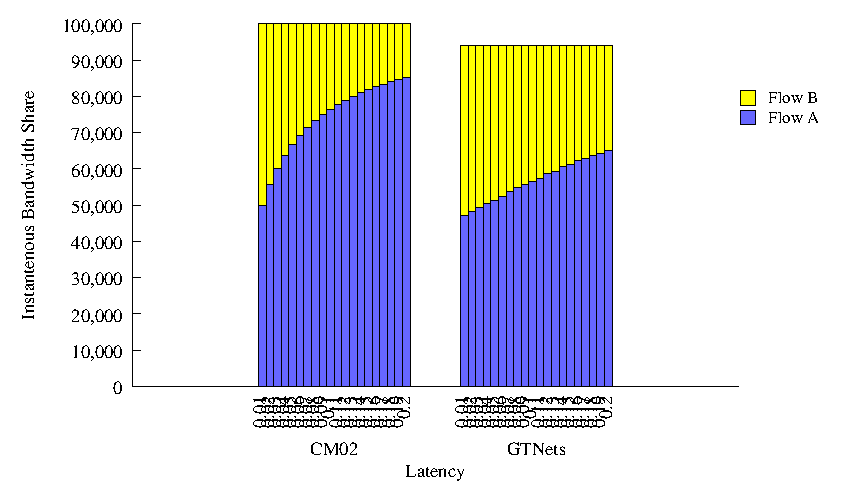
\includegraphics[width=\linewidth]{instantaneous-bw-share-gtnets-vs-cm02.fig}
  \caption{Instantaneous throughput for both flows when the middle
    link is the bottleneck (\BDogbone=100\KB).}
%  FIXME
  \label{fig:sum_throughput}
\end{figure}

On such experiments (see Figure~\ref{fig:sum_throughput}), we can
first remark that the sum of the throughput of both flows is constant
and roughly equal to the bandwidth \BDogbone of the middle link. We
can also observe that the choice of $\alpha=.92$ in the previous section
is also justified by this experiment: the TCP flows only achieve
$92\%$ of the physical bandwidth \BDogbone. 

In such a simple context, the \simgrid model is equivalent to fairly
share the bandwidth \BDogbone between flow $A$ and $B$ with priorities
$w_A=RTT_A$ and $w_B=RTT_B$. Therefore the \simgrid model solves the
following system:
\begin{equation*}
  \begin{cases}
    w_A.\rho_A=w_B.\rho_B \\
    \rho_A + \rho_B = \BDogbone
  \end{cases}
\end{equation*}
Flow $A$ should thus receive $\rho_A = \frac{w_B}{w_A+w_B}\BDogbone$
and flow $A$ should receive $\rho_B =
\frac{w_A}{w_A+w_B}\BDogbone$. Note that when maximizing
$\frac{\sqrt{3/2}}{w_A}\tan^{-1}(\sqrt{3/2}w_A\rho_A)+
\frac{\sqrt{3/2}}{w_B}\tan^{-1}(\sqrt{3/2}w_B\rho_B)$ under the same
constraint, we end up with the exact same sharing. Therefore the
Max-Min sharing algorithm should not be incriminated for computing
inaccurate results. It is the approximation of the weights $w$ by the
round-trip time that results in a bad sharing. Somehow, the simulation
results suggest that this weight should not only account for the
physical latency of the used links but also for their physical
bandwidth. By dividing $\rho_A$ by $\rho_B$ we get the ratio of
priorities $w_A$ and $w_B$, which we can try to model as a function of
$\LDogbone$ and $\BDogbone$. Figure~\ref{fig:gt_ratio_dogbone} depict
this ratio for \gtnets measurements. This function is linear in
$\LDogbone$ and is increasing with an asymptotic value in $\BDogbone$.

\begin{figure}
  \centering
  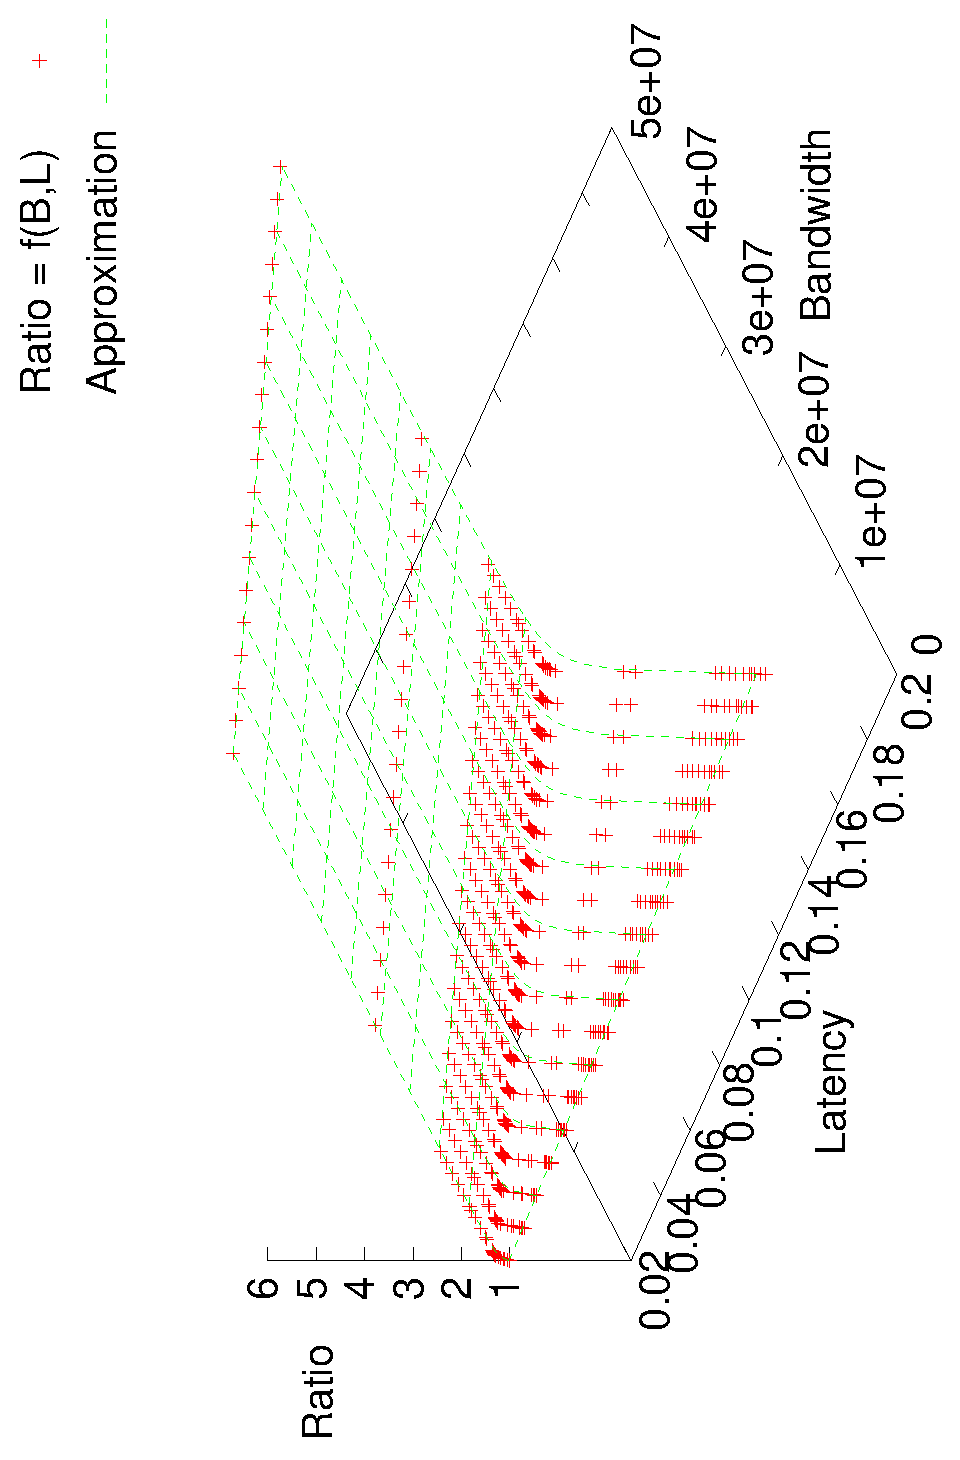
\includegraphics[angle=270,width=\linewidth]{ratio-b-l.fig}
  \caption{Ratio of the throughput for \gtnets as a function of $\LDogbone$ and $\BDogbone$ and its approximation by equation~\eqref{dogbone.apx}.}
  \label{fig:gt_ratio_dogbone}
\end{figure}

In the original \simgrid model, the weight of a flow is computed as
the sum of the physical latencies of the link used by this flow. In
the present example (see Figure~\ref{fig:dogbone}), the \simgrid model
predict the ratio 
$\rho_A/\rho_B$ with the following formula:
\begin{equation*}
  \rho_A/\rho_B = \frac{30+\LDogbone}{40}
\end{equation*}
This formula is indeed linear in \LDogbone but does not account at all
for the dependency on \BDogbone. The measurements in
Figure~\ref{fig:gt_ratio_dogbone} suggest to incorporate the bandwidth
as follows:
\begin{equation}
  \label{eq:sigma}
  w_i= \sum_{k|\F_i \text{ uses } \L_k} \left(Lat_k +
    \frac{\sigma}{B_k}\right),
\end{equation}
which gives us the following model $\rho_A/\rho_B$ in the present example:
\begin{equation}
  \label{dogbone.apx}
  \rho_A/\rho_B = \frac{30+\LDogbone + \sigma\left(\frac{2}{10^8}+
      \frac{1}{\BDogbone}\right)}{
    40 + \sigma\left(\frac{2}{10^8}+
      \frac{1}{\BDogbone}\right)}
\end{equation}
By computing $\sigma$ that minimizes the maximum error on all
flows, we get $\sigma=8775$, the approximation mesh in
Figure~\ref{fig:gt_ratio_dogbone}. This new model improves on the
previous 
model (see Table~\ref{tab.dogbone_comparison}) since it has a maximum
error of 43\% (instead of 200\% for the original model) and an average
error of 4\% (instead of 15\% for the original model). Remember that
these values emphasize the model flaws since they have been computed
by sampling more precisely bandwidth parameters that lead to large
errors (\ie the interval $[0.1,1]$\MBps).
The approximation of $w$ by the
sum of physical latencies had been indeed discussed in the earliest
stages of the development of the \simgrid model~\cite{RR-Loris} and,
as illustrated by Table~\ref{tab.dogbone_comparison},
this approximation holds indeed only when there is little contention.

Therefore we propose the new following model for \simgrid. Each flow
$\F_i$ really starts after $10.4\sum_{k | \F_i \text{ uses } \L_k}
L_k$ and the bandwidth sharing of active flow is computed by solving
the following program:
\begin{LinearProgram}[Maximize]{\min_i w_i.\rho_i}
  \EquationsNumbered{
    \cnstslabel{eq.link_bound_new} \forall \L_k, \sum_{i | \F_i \text{
        uses } \L_k} \rho_i \leq 0.92 B_k\\
    \cnstslabel{eq.flow_bound_new} \forall \F_i, \rho_i \leq \frac{W}{RTT_i}
  }
\end{LinearProgram}
where
\begin{equation*}
  w_i = \sum_{k | \F_i \text{ uses } \L_k} \left(L_k + \frac{8775}{B_k}\right).
\end{equation*}
The error obtained with this new model is summarized on
Table~\ref{tab.dogbone_comparison}.

\section{Random Graphs}
\label{sec.random}

In this section, we reproduce the ``Random Topology'' experiments to
check whether the new model improves on the original \simgrid model in
more general settings than the previous two simple experiments.  To
this end, we have generated four sets of 10 random topologies with the
Waxman model~\cite{Waxman88} and the BRITE generator~\cite{brite}
(Figure~\ref{fig:random} illustrates a typical 50-node random topology). The
sets comprised either small (50 nodes) or large (200 nodes) and either
homogeneous ($B$ follows a uniform distribution in $[100,128]$ \MBps)
or heterogeneous ($B$ follows a uniform distribution in $[10,128]$
\MBps) platforms. The latency is computed by BRITE based on the
Euclidean distance and lies in the interval $(0,5]$\ms in those
experiments. The message size was fixed to $S=10\MB$.
Last, 150 flows were generated between random pairs of end-points in
the topology and 10 different deployments were tried for each
platform. We use the same error model and the same protocol as in the
previous section (\ie all flows are stopped as soon as the first
flow ends and their instantaneous throughput is computed using the
amount of data transfered so far).

\begin{figure}
  \centering
  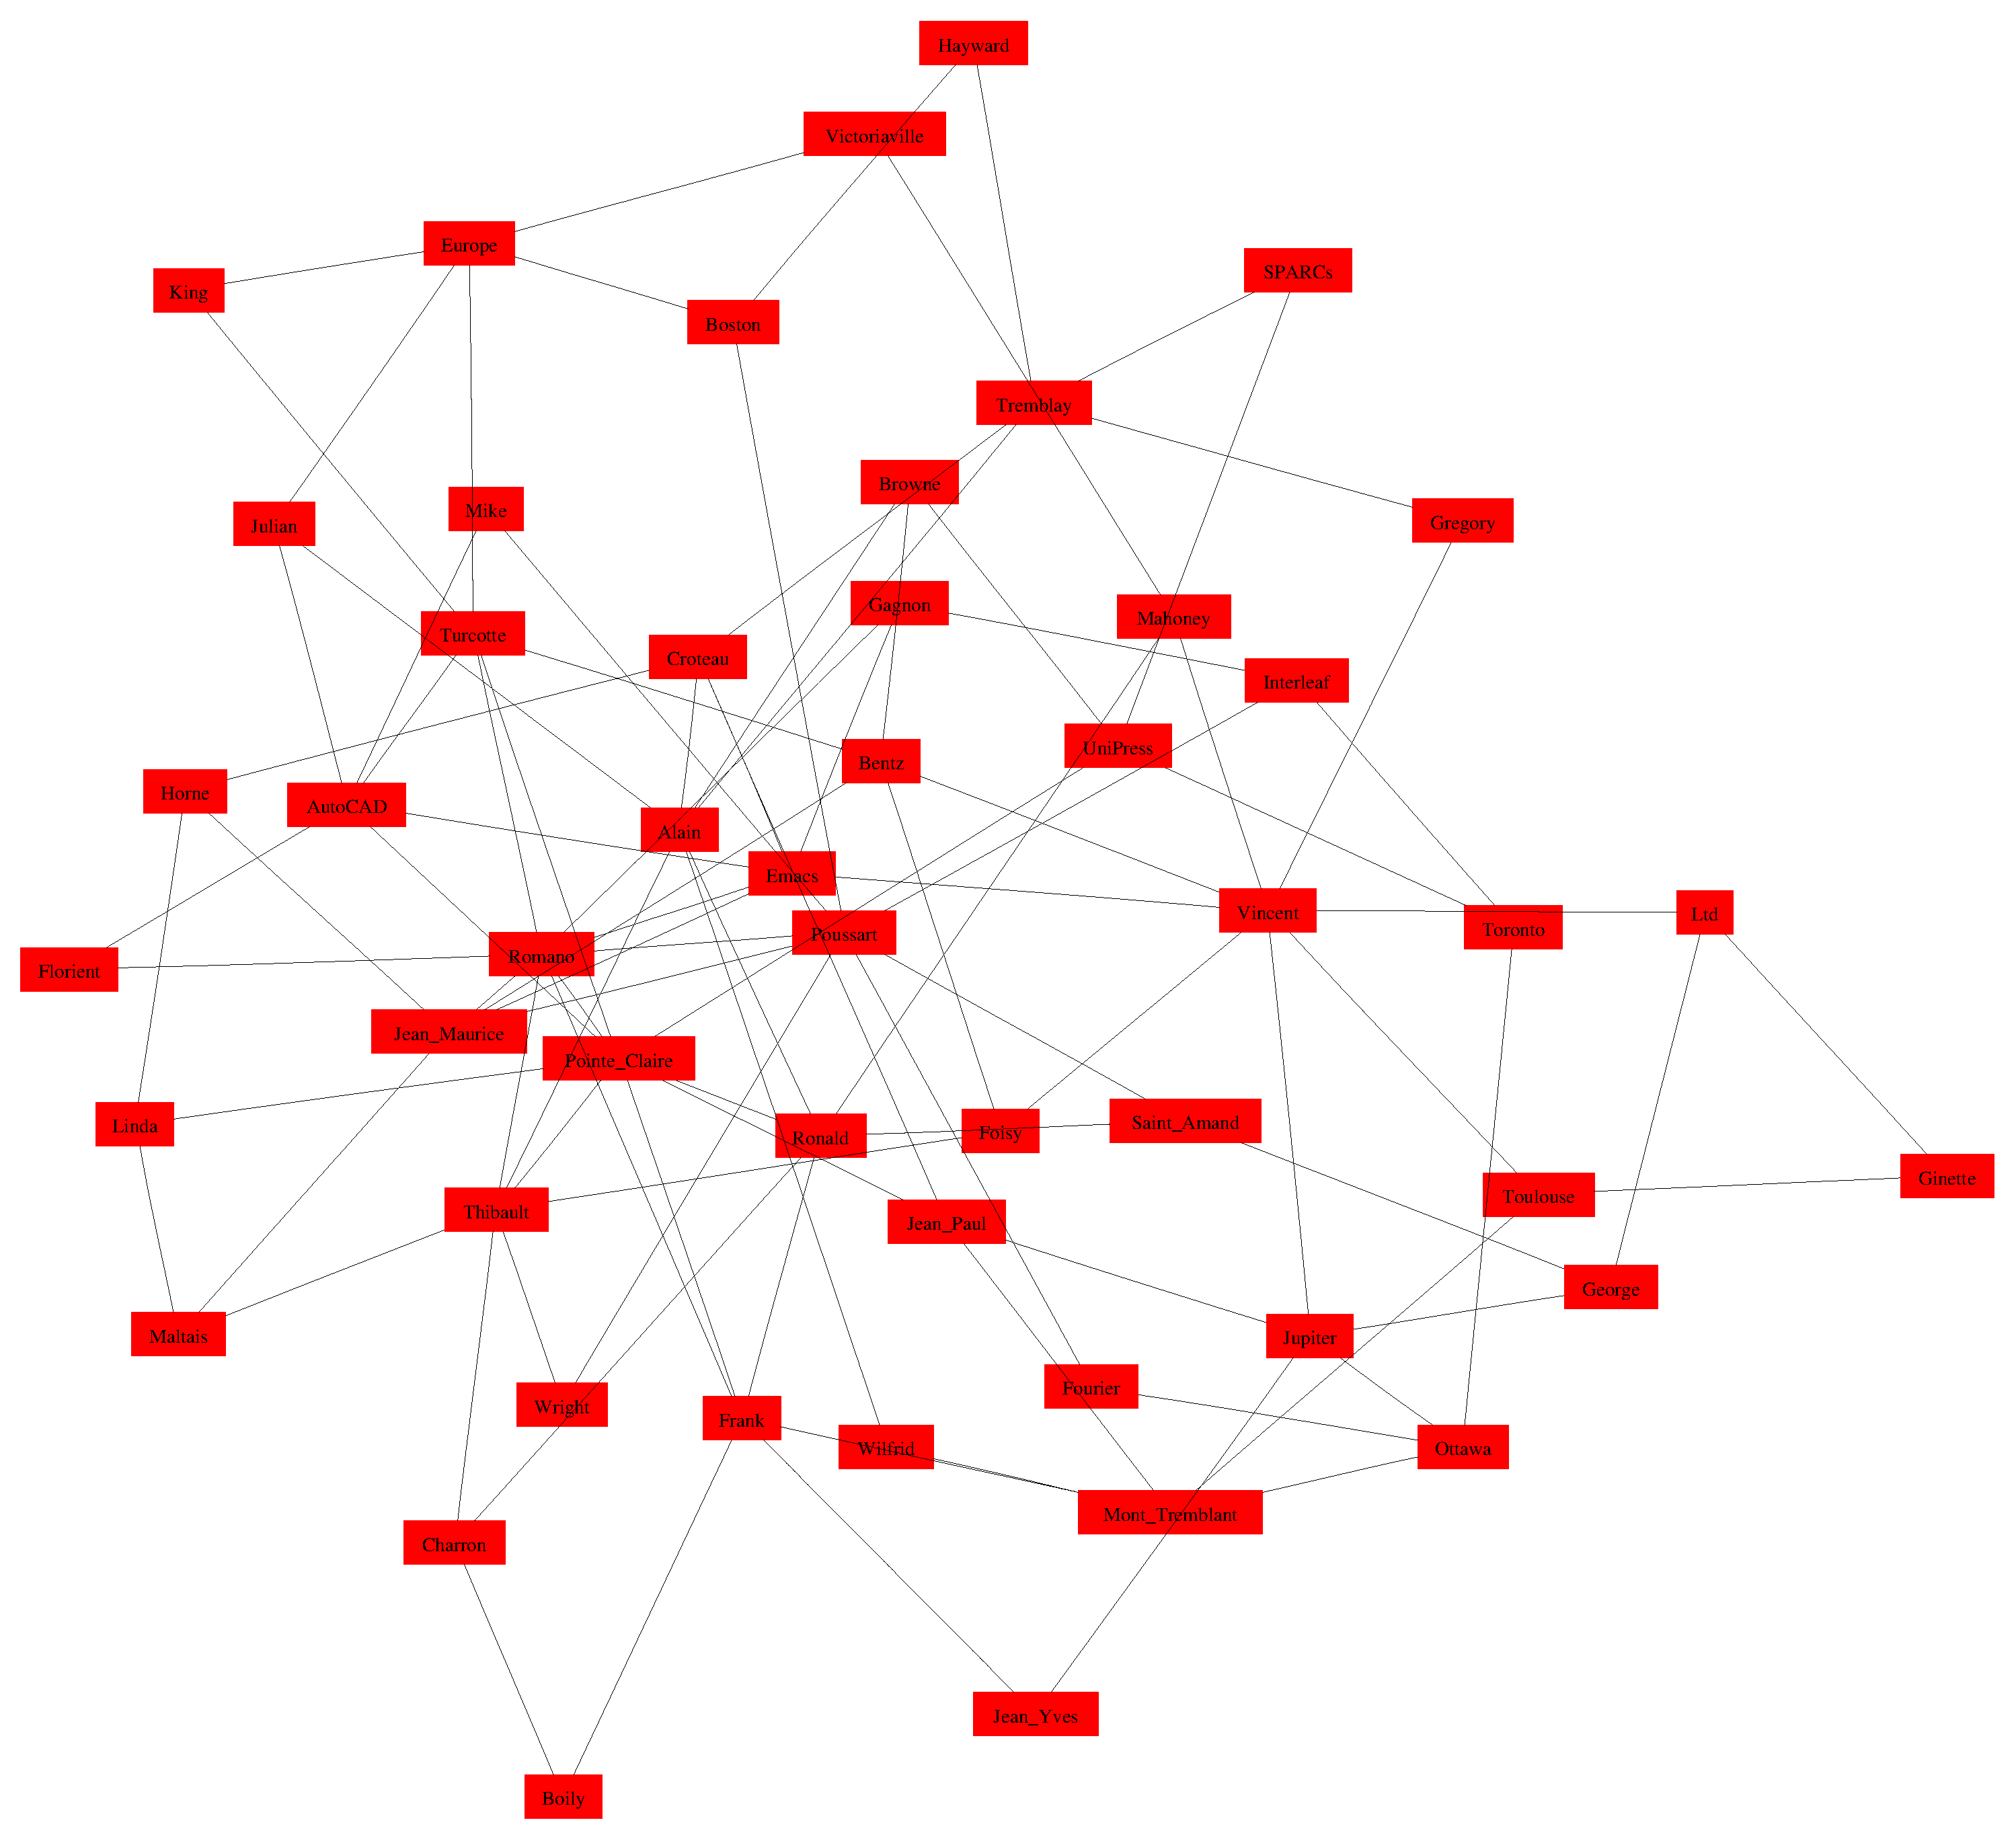
\includegraphics[width=\linewidth]{waxman-platform.eps}
  \caption{Typical 50-node random topology}
  \label{fig:random}
\end{figure}

The lower part of Figure~\ref{fig:random_error_1} depicts the error
distribution obtained for a typical experiment (we have sorted the
flows according to the error of the old \simgrid model). Note that we
haven't applied the absolute value of the logarithmic difference here
to represent underestimation and overestimation.  The upper part
depicts the bandwidth of the corresponding flow for each model. The
lower part depicts the corresponding error when compared to \gtnets 
for each flow in both models.  This
graph confirms the conclusion from~\cite{nstools07}: in the old
\simgrid model high contention (\ie low
bandwidth values) and the error are correlated. It is interesting to see that this
seems to have disappear with the new model: this problem was certainly
due much more to a bad estimation of weights (that we solved in
Section~\ref{sec.dogbone}) rather than to the Max-Min sharing algorithm.

\begin{figure}
  \centering
  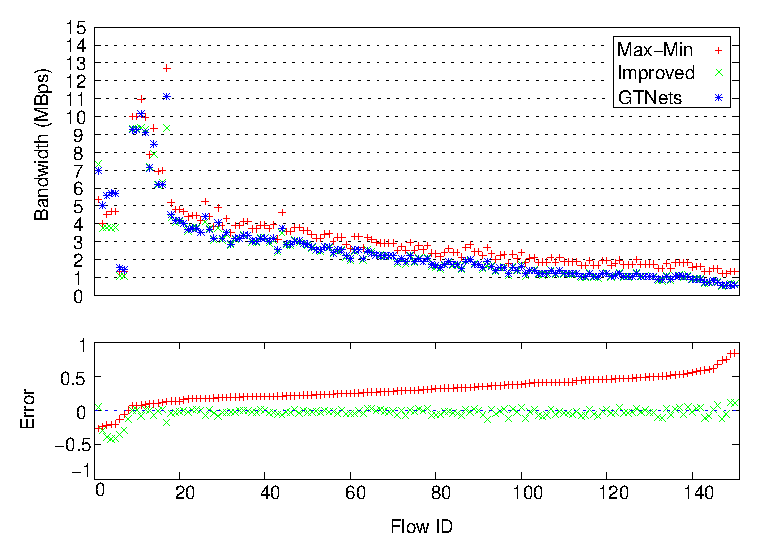
\includegraphics[width=\linewidth]{comparison-gtnets-maxim-improved.fig}
  \caption{Logarithmic errors of both models for a typical
    heterogeneous 50 node random topology.}
%  FIXME
  \label{fig:random_error_1}
\end{figure}

Figure~\ref{fig:random_improvement.a} illustrates the improvement of
the new model versus the previous \simgrid model considering the
mean logarithmic error as metric on the whole set of experiments. The
experiments are sorted according to the error of the new model. The
upper graph depicts the mean error for both models. On the lower
graph, we plot for each experiment the logarithmic ratio between the
mean logarithmic error of the old \simgrid model and the mean
logarithmic error of the new model.  As this logarithmic ratio is
always positive, our new model always improves on the mean logarithmic
error of the previous model (by 234\% on the average). In the end, the
average mean logarithmic error is equal to $0.042$, that is to say
$4\%$.

Figure~\ref{fig:random_improvement.b} is organized in the same way and
illustrates the improvement with respect to the maximum logarithmic
error. This error measure is much harder to improve as it requires to
be accurate on the 150 flows at the same time. Therefore, we do not
succeed to improve on the older model in all situation but still, on
the average, we improve the maximum logarithmic error by 78\%.  In the
end, the average max logarithmic error is equal to $0.32$, that is
to say $38\%$. The largest error with the new model is a situation
where the throughput of one flow is off by $461\%$, which is clearly
still not acceptable. The largest error with the old model is a
situation where the throughput of one flow is off by more than
$534\%$.

\begin{figure*}[ht]
  \centering
  \subfigure[Improvement of the mean logarithmic error.]{
    \label{fig:random_improvement.a}
    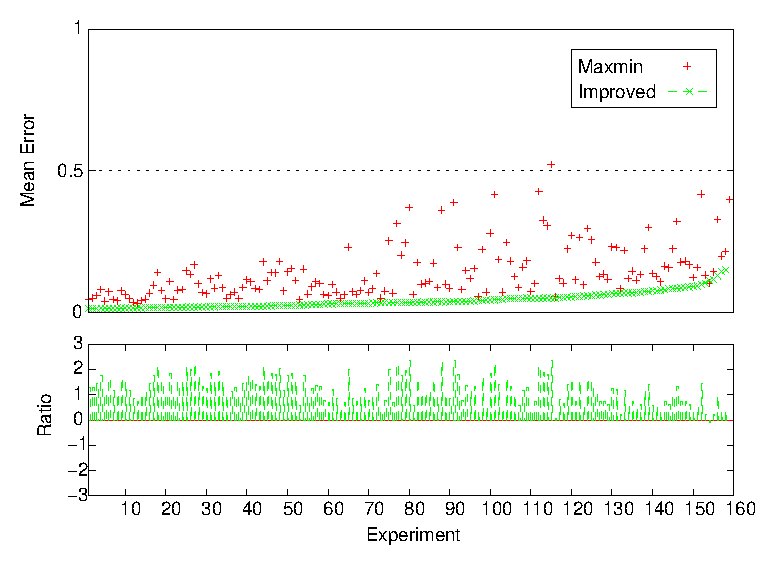
\includegraphics[width=.4\linewidth]{randon-mean.fig}
  }\hfil
  \subfigure[Improvement of the maximum logarithmic error.]{
    \label{fig:random_improvement.b}
    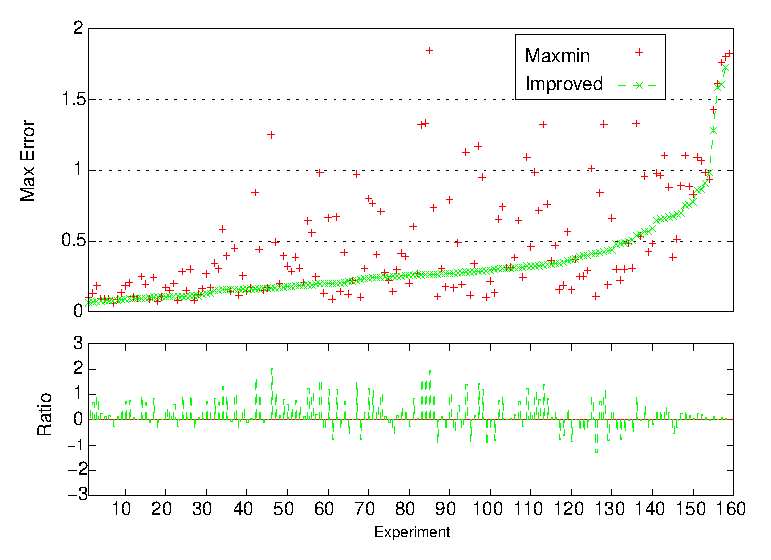
\includegraphics[width=.4\linewidth]{randon-max.fig}
  }
  \caption{Improvement of the logarithmic error for the new model.}
  \label{fig:random_improvement}
%  FIXME
\end{figure*}

The new model is thus much better than the former \simgrid model and
performs well on the average (only $5\%$ of error on the
average). However, there remains situations where it does not accurate 
estimates communication time, particularly for the maximum logarithmic
error metric
(see Table~\ref{tab:random_largest}). Thus, there is still room for
improvement and we believe the Max-Min sharing mechanism can now be
incriminated.

\begin{table*}
\caption{Largest errors in random topology}
\label{tab:random_largest}
\begin{center}
\scalebox{1}{\begin{tabular}{c|c|c|c|c|c|c|c}
\hline
Platform & Exp & \multicolumn{3}{c|}{\simgrid Model
  Logarithmic Error} &
\multicolumn{3}{c}{Improved Model Logarithmic Error} \\ 
\cline{3-8}
         &            & MAX & MEAN & SD  & 
         MAX & MEAN & SD \\ \hline 
waxman\_200\_4.xml & 10 & 0.4921 & 0.1817 & 0.0818 & 0.1689 & 0.0496 &
0.0261 \\
waxman\_200\_2.xml & 8 & 1.8481 & 0.5215 & 0.3070 & 0.2642 & 0.0501 &
0.0499 \\
waxman\_50\_3.xml & 7 & 0.3075 & 0.1406 & 0.0631 & 0.2701 & 0.0224 &
0.0312 \\
waxman\_200\_3.xml & 2 & 0.4589 & 0.1763 & 0.0849 & 0.3226 & 0.0352 &
0.0357 \\
waxman\_200\_1.xml & 9 & 1.3248 & 0.4263 & 0.2430 & 0.3321 & 0.0497 &
0.0576 \\
waxman\_200\_2H.xml & 8 & 1.0135 & 0.3206 & 0.1824 & 0.4118 & 0.0845 &
0.0617 \\
waxman\_50\_1.xml & 5 & 1.3280 & 0.3052 & 0.1981 & 0.4244 & 0.0501 &
0.0553 \\
waxman\_200\_3H.xml & 7 & 0.2238 & 0.1129 & 0.0443 & 0.4840 & 0.0700 &
0.1124 \\
waxman\_200\_4H.xml & 8 & 0.3086 & 0.0761 & 0.0423 & 0.5062 & 0.0315 &
0.0618 \\
waxman\_50\_4.xml & 8 & 1.3322 & 0.4177 & 0.2844 & 0.5406 & 0.0988 &
0.1073 \\
waxman\_50\_2.xml & 3 & 0.9592 & 0.3274 & 0.1935 & 0.5662 & 0.1280 &
0.1040 \\
waxman\_50\_3H.xml & 8 & 1.1057 & 0.2244 & 0.1351 & 0.7531 & 0.0842 &
0.1198 \\
waxman\_50\_2H.xml & 3 & 1.0930 & 0.1625 & 0.1992 & 0.8618 & 0.0791 &
0.1430 \\
waxman\_50\_4H.xml & 3 & 1.4286 & 0.1325 & 0.1687 & 1.2793 & 0.0710 &
0.1833 \\
waxman\_50\_1H.xml & 6 & 1.7615 & 0.1226 & 0.1733 & 1.6041 & 0.0906 &
0.1897 \\
waxman\_200\_1H.xml & 5 & 1.8034 & 0.0969 & 0.2279 & 1.7246 & 0.0573 &
0.2152 \\ \hline
\end{tabular}}
\end{center}
\end{table*}

\section{Conclusion}
\label{sec.conclusion}

In~\cite{nstools07} the \simgrid network engine
was compared to the \gtnets packet level simulator considering the
accuracy/speed tradeoff. In response time, the \simgrid framework cannot
rely on packet level simulation since hundreds of flows lead to an
unacceptable simulation time. Regarding accuracy, conclusions pointed
that the \simgrid network model was good only for messages over 10\MB, due to the TCP slow
start non-linear behavior. Another accuracy flaw was 
detected when the network is highly contended. This last issue
seemed to blame the sharing model in \simgrid, pointing that
future work should experiment different models as those presented
in~\cite{Low03}. 

In the present work, we have shown that the \simgrid model could be
improved to guarantee an excellent accuracy for messages greater than
100\KB (instead of 10\MB). Further investigations pointed that the
issue for highly contended networks was due to a bad instantiation of
the model instead of previous suspicions indicating the sharing model
as the cause.  By correctly instantiating the \simgrid Max-Min sharing
algorithm, we have been able to significantly reduce the error even on
complex platforms and complex communication patterns.

In spite of the successful results presented here, the Max-Min sharing
approach still should be compared to the models proposed
in~\cite{Low03} to ensure that its accuracy cannot be further
improved. Another open research point is the precise determination of
the validity range of this model. Having a more precise knowledge of
the acceptable range of platform parameters provided by \simgrid
end-users would enable to have a much more reliable simulation
framework. The simulator could then warn users when their parameters
are out of range and might even provide interval confidence on the simulation
results. We look forward to present such results in future work.

\section*{Acknowledgement}
We would like to thank Henri Casanova and Kayo Fujiwara for their
trailing work in integrating \gtnets in the \simgrid kernel and for
their preliminary study on the validity of \simgrid's
models~\cite{nstools07}. We also thank them for letting us access
their experimental data and letting us reproduce the related work
section. 

Experiments presented in this paper were carried out using the
Grid'5000 experimental testbed, an initiative from the French
Ministry of Research through the ACI GRID incentive action, INRIA,
CNRS and RENATER and other contributing partners (see \url{https://www.grid5000.fr}).

This work is partially supported by ANR ({\it Agence National de
  Recherche}), project reference ANR 08 SEGI 022. Special thanks to
CAPES/Brazil which supports Pedro Velho's PhD thesis 
during the presented work.  



\bibliographystyle{abbrv}
\bibliography{validation_simutools}



\end{document}



% Local IspellDict: american
